\documentclass[english, fontsize=12pt, paper=a4, twoside=false, draft=true, pagesize=auto, version=last, DIV=16]{scrartcl}


\let\counterwithout\relax
\let\counterwithin\relax

\usepackage[utf8]{inputenc}
%Für Tabellen
\usepackage{tabularx}

% Für Absätze in Bildbeschreibung
\usepackage{caption}

% Zur nummerierten Aufzählung, mit automatischem Einrücken
\usepackage{paralist}
\usepackage{enumitem}
\usepackage{csquotes}


% mitwachsender Implikationspfeil mit Text
\makeatletter
\newcommand{\xRightarrow}[2][]{\ext@arrow 0359\Rightarrowfill@{#1}{#2}}
\makeatother


% Java Code Einbinden
\usepackage{listings}
\usepackage{color}
\usepackage[svgnames]{xcolor}



% Um einzelne Seiten zu drehen
\usepackage{pdflscape}
%\usepackage{rotating}
%\usepackage{lscape}


\usepackage{lmodern}
\usepackage[T1]{fontenc}
%\usepackage[latin1]{inputenc}
\usepackage{babel}
\usepackage[utf8]{inputenc}
\usepackage{stmaryrd}
\usepackage{extarrows}
\usepackage{ulem}



%Zur Bildnummerierung
\usepackage{chngcntr}
\usepackage{mathtools}
\usepackage{amsmath}
%Zur Verwendung von "chngcntr": \counterwithin{figure}{section}


%Euro-Zeichen
\usepackage{eurosym}

\usepackage{float}

\usepackage{amsmath}
\usepackage{acronym} %[''Optionen'']
\usepackage{esvect}  %Für Vektorpfeile, Aufruf mit \vv{Vektorname}

% Für schön Buchstaben1
\usepackage{mathrsfs}
\usepackage{suetterl}
\usepackage{calligra}

%%% Neue Kommandos/Begriffe %%%
%\renewcommand{\thesection}{\arabic{section}}
% Für Fußnoten ohne Nummer
%\renewcommand{\thefootnote}{}



% Für die Normalschrift im Abkürzungsverzeichnis, das Paket "acronym" veranlasst eine andere Schriftart bei Abkürzungen.
\newcommand{\Rule}{\rule{\textwidth}{0.5mm}}
% \newcommand{\absatzParagraph}[1]{\paragraph{#1}\mbox{}\\}


\usepackage{geometry}
\newgeometry{left=18mm,right=18mm,top=15mm,bottom=15mm}
\footskip = 22pt

\usepackage{setspace}  % Paket einbinden
\onehalfspacing        % einstellen des Zeilenabstandes auf 1,5
\setlength{\parindent}{0in}
\usepackage{amsmath}
\usepackage[amsmath,amsthm,thmmarks]{ntheorem}
\usepackage{amssymb}


% Komplexitätsklassen
% \usepackage[bold,full]{complexity}


% Für Pseudocode
\usepackage{algorithm}
\usepackage{algpseudocode}


% für mehrzeilige Kommentare
\usepackage{verbatim}


% ------------- Beginn Definition von: Satz, Lemma Definition usw. -------------
\theoremstyle{break}
%\theoremstyle{definition}
\theorembodyfont{\upshape}
\newtheorem{defin}{Definition}[section] % Präambel
\newtheorem{lemma}[defin]{Lemma}
\newtheorem{satz}[defin]{Satz}
\newtheorem{kor}[defin]{Korollar}
\newtheorem{beo}[defin]{Beobachtung}
\newtheorem{bemerk}[defin]{Bemerkung}
\newtheorem{übung}[defin]{Übung}

%  ------------- Ende Definition von: Satz, Lemma Definition usw. -------------

% Für URLs
\usepackage{url}
\usepackage{hyperref}
\hypersetup{final}



\usepackage{animate}
\usepackage{graphicx}
\usepackage{graphics}
\usepackage{hyphenat}


\usepackage{tikz}
\usepackage{tkz-euclide}
%\usepackage{tikz,fullpage}
\usetikzlibrary{calc,patterns,through,intersections}
%\usepackage{tkz-berge}

\newcommand*\bigO{\mathcal{O}}



\begin{document}


\title{
\vspace*{-10mm}
Exercise 3 \\[-3pt]
{\Large $\mathrm{for \ the \ lecture}$} \\[-3pt]
{\LARGE \textbf{Computational Geometry}}
}
\author{Dominik Bendle, Stefan Fritsch, Marcel Rogge and Matthias Tschöpe}
\maketitle
\vspace*{-10mm}

\section*{Exercise 1 (Doubly-Connected Edge List)}
\textbf{a)} Which of the following equations are always true?. 
\begin{align}
\text{Twin}(\text{Twin}(\vec{e})) = \vec{e} \\
\text{Next}(\text{Prev}(\vec{e})) = \vec{e} \\
\text{Twin}(\text{Prev}(\text{Twin}(\vec{e}))) = \text{Next}(\vec{e}) \\
\text{IncidentFace}(\vec{e}) = \text{IncidentFace}(\text{Next}(\vec{e}))
\end{align} \par
\medskip
(1) True. See definition of Twin. \\
(2) True. See definitions of Prev and Next. \\
(3) False. Consider figure \ref{fig:task_1_example} as counterexample, with $\vec{e} := \vec{e}_{2,2}.$
\begin{align*}
&\text{Twin}(\text{Prev}(\text{Twin}(\vec{e}))) \\
= &\text{Twin}(\text{Prev}(\text{Twin}(\vec{e}_{2,2})))\\
= &\text{Twin}(\text{Prev}(\vec{e}_{2,1})) \\
= &\text{Twin}(\vec{e}_{4,2}) \\
= & \vec{e}_{4,1}\\
\neq & \vec{e}_{3,1}\\
= &\text{Next}(\vec{e}_{2,2}) \\
\end{align*}

(4) True. See defintion of IncidentFace. \\

\vspace*{10mm}
\newpage
\begin{figure}[t]
\centering
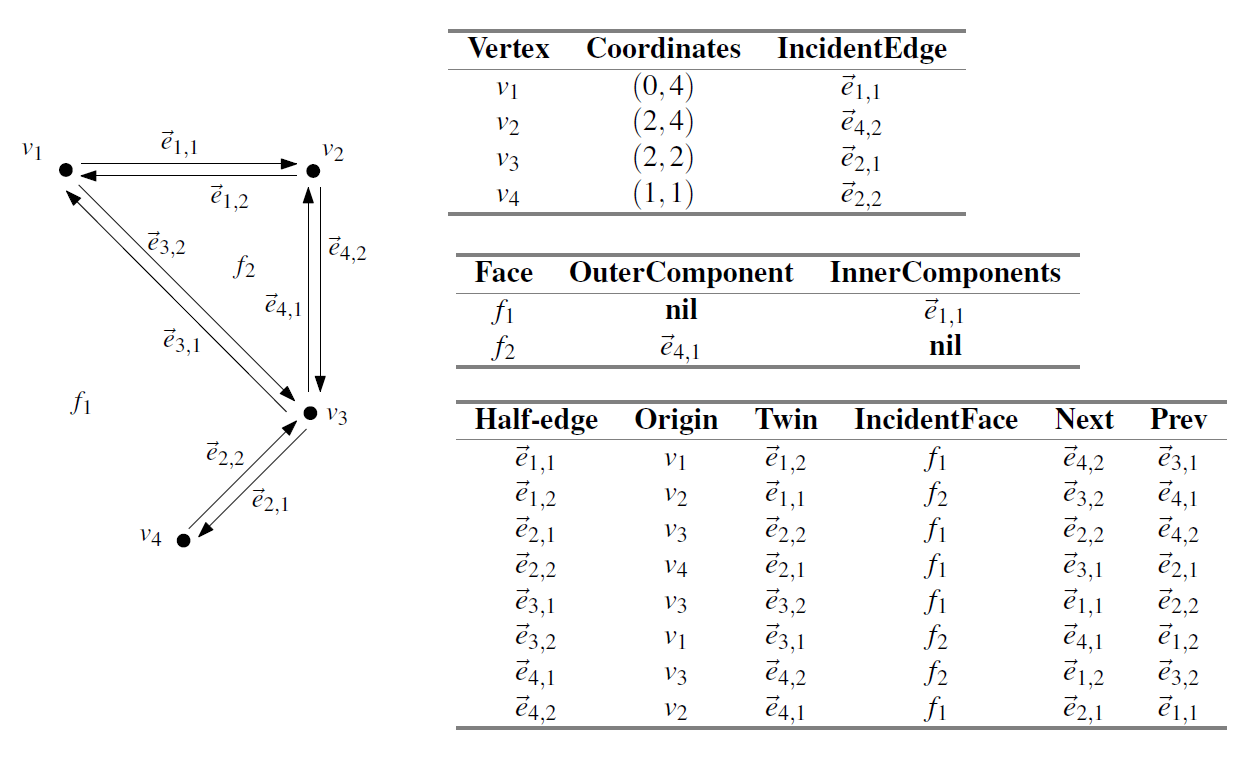
\includegraphics[width=\textwidth]{images/task_1_example.png}
\caption{An example of a doubly-connected edge list for a simple subdivision. Figure is taken from \cite{berg2008computational}.}
\label{fig:task_1_example}
\end{figure}

\textbf{b)} Give an example of a doubly-connected edge list where for an edge $\vec{e}$ the faces IncidentFace($\vec{e}$) and IncidentFace(Twin($\vec{e}$)) are the same. \par
\medskip
Consider this example: \\
\begin{figure}[h]
\centering
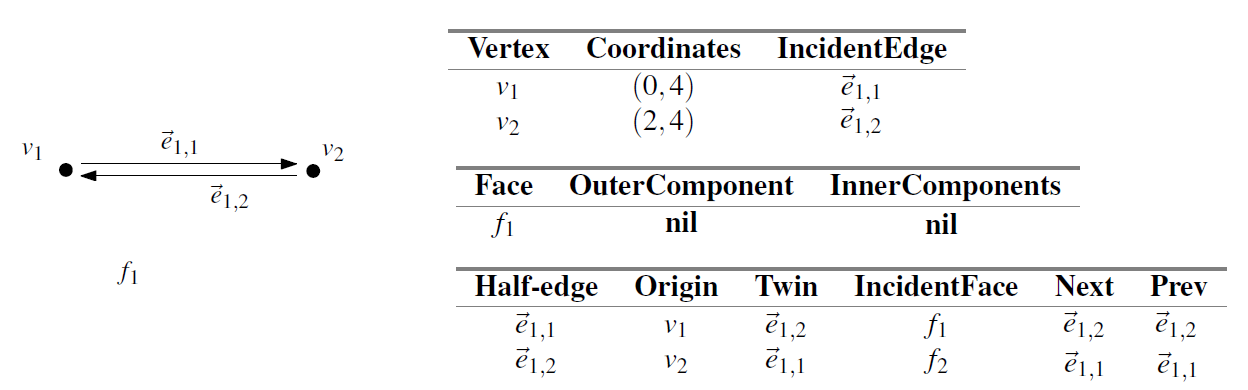
\includegraphics[width=\textwidth]{images/task_1_b.png}
\label{fig:task_1_b}
\end{figure}

This is a doubly-connected edge list where $f_1 = \text{IncidentFace}(\vec{e}_{1,1}) = \text{IncidentFace}(\text{Twin}(\vec{e}_{1,1})) = \text{IncidentFace}(\text{Twin}(\vec{e}_{1,2})) = \text{IncidentFace}(\vec{e}_{1,2}) = f_1 $ holds.

\vspace*{10mm}
\textbf{c)} Given a doubly-connected edge list representation for a subdivision where
\begin{align*}
\text{Twin}(\vec{e}) = \text{Next}(\vec{e})
\end{align*} 
holds for every half-edge $\vec{e}$. How many faces can the subdivision have at most? \par
\medskip

\vspace*{10mm}
\newpage




\section*{Exercise 2 (Planar Subdivision and Point Set)}


\newpage

%
% ---- Bibliography ----
%
\bibliographystyle{plain}
\bibliography{bib}
%
\end{document}



